\documentclass{article}
\usepackage{microtype}
\usepackage{graphicx}
\usepackage{subcaption}
\usepackage{booktabs}
\usepackage{hyperref}
\newcommand{\theHalgorithm}{\arabic{algorithm}}
\usepackage{icml2027}
\usepackage{amsmath}
\usepackage{amssymb}
\usepackage{mathtools}
\usepackage[capitalize,noabbrev]{cleveref}
\graphicspath{{../figtab/}}

\newcommand{\phis}{\phi^{\star}}
\newcommand{\phih}{\hat\phi}
\newcommand{\topk}{\mathrm{top}_k}

\icmltitlerunning{Is one SHAP run enough?}

\begin{document}

\twocolumn[
  \icmltitle{Is one SHAP run enough? A budget-indexed, decision-level\\
  reliability audit of single-run Shapley attributions on tabular models}
  \icmlsetsymbol{equal}{*}
  \begin{icmlauthorlist}
    \icmlauthor{Anonymous Authors}{anon}
  \end{icmlauthorlist}
  \icmlaffiliation{anon}{Anonymous Institution}
  \icmlcorrespondingauthor{Anonymous Authors}{anon@example.com}
  \icmlkeywords{Shapley values, explanation reliability, tabular data}
  \vskip 0.3in
]
\printAffiliationsAndNotice{}

\begin{abstract}
Tabular models are routinely explained by running a sampling-based Shapley estimator once and reporting the top few attributes. When is that single run reliable evidence for the explanation of that prediction, and can the deployer tell from the run? We measure, per instance and at the level of the reported top-$k$ set, how often a run reproduces the exact interventional Shapley top-$k$, keeping repeatability across reruns apart from accuracy against the exact value, and we audit in-run certificates on fresh reruns. On two public tasks ($d=16$ and $d=20$) and three model classes, the shipped KernelSHAP default returns the exact top-3 set in 97\% of runs on average on ACS Employment, with a 7--10\% tail of near-tie instances, but in only 83--88\% on German Credit. There the error is repeatable, is not cured by sixteen times the budget, and comes from the default's $\ell_1$ feature selection; switching it off at the same budget gives 97--99\%. Four of five in-run certification rules are calibrated, but they are conservative, and cost at least about forty times what a fixed corrected estimator needs for the same exact rate, which gives no per-run statement.

\end{abstract}

\section{Introduction}
\label{sec:intro}

A bank that declines a loan, or a clinic that flags a patient, is often asked for the reasons. For a tabular model the usual answer is the few attributes with the largest Shapley attributions, obtained by running a sampling-based estimator such as KernelSHAP \citep{lundberg2017unified} once on that instance, at the library's default budget, and reporting the top of the list. The estimator is random and its budget is limited, so a second run may report different reasons. Two attributions with nearly equal magnitude may swap, and a systematic error in the estimator may place the wrong attribute in the set in every run. Explanations are checked rarely, and when they are, it is usually by the mean error over many instances.

We ask when a single run is reliable evidence for the explanation of \emph{that} prediction, and whether a deployer can tell from the run itself. We keep two things apart. \emph{Repeatability} asks whether a rerun would report the same attributes; \emph{accuracy} asks whether the run reports what the exact Shapley value would. The first can be measured without the exact value, but the second is what a reason is for, and an estimator can be repeatable without being accurate.

Work on Shapley estimation bounds errors of the full attribution vector \citep{chen2023algorithms,musco2024leverage}, and a few methods give guarantees for identifying the top-$k$ attributes and stop sampling when these hold \citep{covert2021improving,kariyappa2024shapk,goldwasser2024significance,kolpaczki2025antithetic}. Studies of explanation stability and disagreement concern the variation of the explained quantity itself, such as the choice of background \citep{yuan2022background} or of another explainer \citep{krishna2022disagreement}. What is missing for tabular models is a decision-level, per-instance measurement of how often one run of the \emph{shipped} estimator reports the right top-$k$ set, how this depends on the model, the dimension and the budget, and whether the in-run certificates that exist can be trusted when used as intended.

We provide this measurement. Our approach has three parts. First, we measure reliability per instance and at the decision level: for each instance, the probability $r_k$ that a run returns exactly the top-$k$ set of the exact interventional Shapley value, estimated from repeated runs, and the fraction of instances for which this probability is at least $1-\delta$; the reference is computed exactly by enumeration. Second, we read these numbers against explicit scales: chance, the gap between the $k$-th and $(k{+}1)$-th attribution relative to the estimator's standard error, and the variation that practitioners already accept from resampling the background and from retraining. Third, we audit certificates from the literature for calibration on fresh reruns, under the stopping rule they prescribe.

On two public tasks, three model classes and three seeds, we find:
\begin{itemize}
\item \textbf{The mean hides a tail, and a default fails repeatedly.} On ACS Employment ($d=16$) the shipped KernelSHAP returns the exact top-3 set in 97\% of runs on average, but 7--10\% of instances are unreliable; these are near ties, and the top-3 is correct up to a 10\% tolerance in essentially every run. On German Credit ($d=20$) the same default is correct in only 83--88\% of runs. The error is repeatable (rerun stability 0.95--0.97), it is not cured by sixteen times the budget, and it comes from the default's $\ell_1$ feature selection; switching selection off at the same budget gives 97--99\%.
\item \textbf{Certificates are calibrated but conservative, and dear.} Four of five certification rules deliver at least their nominal level on fresh reruns; the fifth, which tests the boundary pair on the run's own estimate, over-claims for the larger $\delta$ and $k$ in three of six cells. The calibrated rules abstain on 22--76\% of the instances an oracle would certify at four times the default budget, and cost at least about forty times what a fixed corrected estimator needs for the same exact rate (the fixed estimator is at the floor of our budget grid, and makes no per-run statement).
\end{itemize}
These findings give the verdict its form: one run suffices for a corrected estimator at a small budget on these models, not for the shipped default at $d=20$, and which instances of the remaining few percent are affected cannot be read from the run without a certificate.

Our contribution is the audit and its evidence, not a new estimator or certificate. We release the code, the exact reference values and all result files with this submission.

\section{Related Work}
\label{sec:related}

\textbf{Estimating Shapley attributions.}
KernelSHAP casts Shapley estimation as a weighted regression over sampled coalitions \citep{lundberg2017unified}; \citet{covert2021improving} analyse it, give an unbiased variant and a per-feature uncertainty estimate with a convergence criterion. Permutation sampling with antithetic, stratified or orthogonal variance reduction \citep{mitchell2022sampling}, paired sampling \citep{mayer2025paired}, leverage-score sampling with provable error \citep{musco2024leverage} and reweighting of the KernelSHAP kernel \citep{olsen2025weighting} reduce error at a given budget; \citet{chen2023algorithms} survey the families, and TreeSHAP computes the value exactly for tree ensembles \citep{lundberg2020trees}. These works bound or reduce the error in the attribution vector. We ask what that error does to the \emph{reported explanation} of a single instance at the budgets in use, which of these remedies the answer requires, and whether the library defaults already suffice.

\textbf{Which value is estimated.}
The attribution depends on how absent features are marginalised \citep{sundararajan2019many,kumar2020problems,chen2020true}. We fix the interventional value for an explicit background sample and treat the choice of that sample as a source of variation separate from estimator noise.

\textbf{Top-$k$ identification with guarantees.}
Closest to our certificate audit are procedures that decide when a sampled attribution identifies the top-$k$ features: SHAP@k gives PAC stopping rules for the top-$k$ set \citep{kariyappa2024shapk}, \citet{goldwasser2024significance} test the significance of feature-importance rankings under instability, and \citet{kolpaczki2025antithetic} design antithetic sampling for top-$k$ Shapley identification. We construct no new rule. We measure whether such rules, and the standard-error and split-half rules built from \citet{covert2021improving}, deliver their nominal level on real tabular models with the library's explainer, on reruns not used to certify, and what they cost against a fixed budget.

\textbf{Stability and disagreement of explanations.}
\citet{krishna2022disagreement} study disagreement between different explanation methods on the same model; \citet{yuan2022background} relate background-set size to SHAP stability for deep models; \citet{alvarezmelis2018robustness} study sensitivity to input perturbation; repeat-run instability and its remedies are studied for LIME \citep{zhang2019trust,visani2020optilime,zhou2021slime}. \citet{marx2019multiplicity} show that equally accurate models disagree on individual predictions, which we use as a yardstick: estimator noise matters in practice to the extent that it exceeds variation a practitioner already cannot remove. Our stability measures follow \citet{nogueira2018stability} and \citet{webber2010rbo}.

\textbf{What these leave open.}
For tabular models, no systematic same-model, same-instance, repeat-run study of SHAP exists that varies dataset, model class, explainer, budget and dimension together, reports per-instance decisions rather than mean error, separates repeatability from accuracy, and compares against chance, margin, background and retraining variation. Nor has the calibration of in-run certificates been examined on fresh reruns at deployed budgets.

\section{Setup and Definitions}
\label{sec:setup}

\textbf{Runs and budget.}
Let $f$ be a trained model, $x$ an instance, $D$ a background sample of size $m$, and $E$ an explainer. A \emph{run} returns $\phih=E(f,x,D,B,\xi)$ with random seed $\xi$. The players are the original attributes (a categorical attribute that is one-hot encoded is masked as one player). The \emph{budget} $B$ is the number of masked-input model evaluations, i.e.\ sampled coalitions times $m$; this is the same unit for every explainer, and wall-clock time is reported next to it. The \emph{default} budget is the one the library chooses when the user gives none.

\textbf{Target.}
The target $\phis$ is the exact interventional Shapley value of the same $(f,x,D)$: by enumeration of all $2^d$ coalitions, in closed form for linear models, and by interventional TreeSHAP for tree ensembles. Whether a run is judged against $\phis$ (accuracy) or against another run (repeatability) is stated for every result.

\textbf{Read-outs.}
What a deployer reports is a decision-level object: the top-$k$ set $\topk(\phih)$ by $|\phih|$ for $k\in\{1,3,5\}$, the signs of these features, their order (compared with RBO), and the reason codes, i.e.\ the top-$k$ among contributions toward the adverse outcome. Because near ties make an exact set a harsh criterion, we also report an $\epsilon$-tolerant version, which counts a set as correct when it differs from $\topk(\phis)$ only in features whose attribution lies within $\epsilon|\phis|$ of the cut. We also report the full vector (relative $\ell_2$ error, cosine).

\textbf{Repeatability and accuracy.}
\emph{Repeatability} is agreement between reruns of the same explainer (chance-corrected set stability \citep{nogueira2018stability}, RBO, top-$k$ Jaccard) and needs no $\phis$. \emph{Accuracy} is the probability that a run reproduces the exact read-out, $r_k(x;B)=\Pr_\xi[\topk(\phih)=\topk(\phis)]$. The two come apart when an explainer is repeatably wrong, as when finite-budget bias or $\ell_1$ feature selection fixes the same error in every run; we decompose the gap into bias and variance.

\textbf{Reliable single run.}
A single run of $E$ is \emph{reliable at $(k,1-\delta)$} for instance $x$ iff $r_k(x;B)\ge 1-\delta$. Our headline quantity is the \emph{fraction of instances} for which this holds, with the distribution of $r_k$ over instances, not its mean.

\textbf{Scales for judging the numbers.}
A disagreement figure has no meaning alone. We read it against (S1) chance: random attributions, another instance's attribution, chance-corrected stability; (S2) the gap scale: the estimator standard error against the gap between the $k$-th and $(k{+}1)$-th attribution, $z=\text{gap}/\mathrm{SE}$; (S3) variation practitioners already live with: per-instance differences between rerun disagreement and the disagreement from resampling the background and from retraining the model (a retrain changes the model, so S3 only says whether estimator noise is smaller or larger than variation already accepted); (S4) budget-matched alternatives: one run at $B$ against the average of $R$ runs at $B/R$, and other estimators at equal $B$; (S5) a global-importance control, the stability of mean $|\phi|$ over many instances.


\textbf{Certificates under audit.}
A run can carry its own evidence. The unbiased KernelSHAP estimator of \citet{covert2021improving} returns a standard error per attribute from the same coalitions, which supports a test that the chosen top-$k$ set separates from the rest. We audit five rules, all computed from one run's coalitions and applied after each stage of a doubling schedule of the budget (from $\tfrac14$ to $16$ times the default), stopping at the first stage that certifies. \emph{Naive} tests only the pair formed by the weakest chosen and the strongest excluded attribute; it uses the selection to define the test and is exposed to the winner's curse. \emph{Bonferroni} and \emph{max-$t$} test all $k(d-k)$ pairs, the second with a simultaneous critical value from the run's estimated covariance. \emph{Split-half} selects the set on one half of the coalitions and tests it on the other, so that selection and test are independent. \emph{SHAP@k-style} stopping applies the interval-separation rule of \citet{kariyappa2024shapk} with $\delta/d$ per attribute. A rule is \emph{calibrated at level $\delta$} if, among runs it certifies, the fraction whose top-$k$ equals $\topk(\phis)$ is at least $1-\delta$; this is measured on fresh reruns, at the stage where each run stopped, so that the winner's curse, multiplicity and optional stopping all count against the rule. Certification is compared with a fixed budget at equal pooled correct rate.

\section{Experiments}
\label{sec:experiments}

\subsection{Experimental setup}
\label{sec:exp-setup}

\textbf{Data and models.}
We use two public tabular tasks small enough for exact reference values: German Credit ($d=20$ attributes, 1000 rows, bad-credit label) and the ACS Employment task for Alabama in 2018 ($d=16$, \citealt{ding2021retiring}); the dependence on $d$ comes from explaining a fixed random subset of the attributes of each dataset ($d=8$ and $12$, one draw each, besides the full set). Nominal attributes are one-hot encoded for the model and masked as one player. Three model classes are explained on the probability scale: logistic regression, a two-layer MLP, and gradient-boosted trees (LightGBM), each with three model seeds; for logistic regression the seeds do not change the model. Each cell explains 100 test instances against a background of $m=30$ training rows, and $\phis$ is computed from the full table of $2^d$ coalitions for the same background. Some attributes equal the background value for an instance; as in the library, they are not players and receive zero.

\textbf{Explainers and budgets.}
The arms are KernelSHAP as shipped in \texttt{shap} 0.51.0 (default $2d{+}2048$ coalitions; with ten or more players its $\ell_1$ rule keeps ten attributes and sets the rest to zero, even when all coalitions are enumerated), KernelSHAP with $\ell_1$ selection off, the unbiased Covert--Lee estimator with standard error, and \texttt{PermutationExplainer} at its shipped default and at matched budgets. All are re-implemented on a common table of exact coalition values and checked against the library itself before use (Appendix~\ref{app:e0}). Each (instance, arm, budget) is rerun $R=20$ times at budgets from $\tfrac14$ to $16$ times the default; about 30 instances per cell are rerun 200 times for statements about single instances. Intervals are cluster bootstrap over instances with model seeds as a second level, and Clopper--Pearson for a single instance's $r_k$. The decision rules that turn each claim into ``supported'', ``not supported'' or ``depends'' were fixed before the runs and are in the released protocol.

\begin{figure*}[t]
\centering
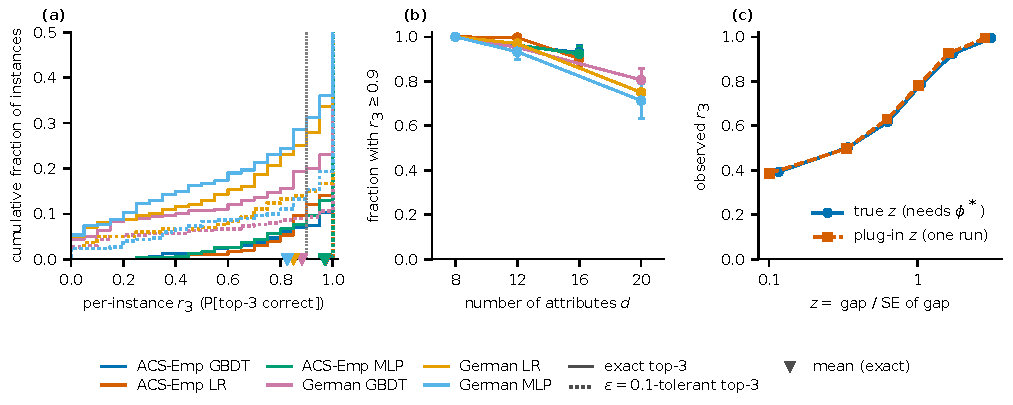
\includegraphics{fig1_tail.pdf}
\caption{\textbf{The mean hides a tail of instances whose top-3 a single run often misses.}
(a)~Empirical CDF over instances of $r_3$, the probability that the top-3 features of a single run equal those of the exact Shapley values,
at the shipped KernelSHAP budget, for the exact top-3 (solid) and the $\epsilon$-tolerant top-3 (dotted; a set counts as correct if it differs from the exact top-3 only in features whose attribution lies within a relative $\epsilon=0.1$ of the cut), one colour per dataset and model;
triangles mark the mean of the exact $r_3$; the thin vertical line is $r_3=0.9$. Only the lower part of the CDF is drawn.
On ACS the exact tail is almost entirely ties (the $\epsilon$-tolerant curves lie at the bottom); on German it is not.
(b)~Fraction of instances with $r_3\ge 0.9$ against the number of attributes $d$ (feature subsets of each dataset), shipped budget, with 95\% cluster-bootstrap intervals.
(c)~Observed $r_3$ against $z$, the gap between the $k$th and $(k{+}1)$th attribution in units of its standard error, binned by quantile (Covert--Lee runs at the shipped budget):
with the true $z$ (needs the exact values) and with the plug-in $z$ of a single run.
$r_3$ from $R{=}20$ reruns per instance; 100 instances per cell, three model seeds.}
\label{fig:tail}
\end{figure*}

\begin{table*}[t]
\caption{\textbf{Reliability of single runs per explainer.}
$F_3$: fraction of instances with $r_3\ge 0.9$ (95\% cluster-bootstrap interval over seeds, then instances); mean $r_3$; Nogueira stability of the top-3 across reruns;
$F_3^{\epsilon}$ and mean $r_3^{\epsilon}$: the same with the $\epsilon$-tolerant top-3 ($\epsilon=0.1$); bias share: share of the unreliable instances whose \emph{mean} attribution over reruns already has the wrong top-3 (a repeatable but wrong explanation). The \texttt{l1\_reg=False} row is the paired variant.
Budget: the shipped KernelSHAP default ($2d+2048$ coalitions) for the KernelSHAP rows and Covert--Lee, $500$ for Permutation.
100 instances per cell, three model seeds, $R{=}20$ reruns.}
\label{tab:reliable}
\centering\small
\begingroup\setlength{\tabcolsep}{2.5pt}
\begin{tabular}{@{}llcccccc@{}}
\toprule
Dataset, model & Explainer & $F_3$ & $F_3^{\epsilon}$ & mean $r_3$ & mean $r_3^{\epsilon}$ & Nogueira & Bias share \\
\midrule
ACS-Emp GBDT & KernelSHAP (shipped) & 0.93 [0.90, 0.96] & 1.00 [1.00, 1.00] & 0.97 & 1.00 & 0.99 & 0.10 [0.00, 0.24] \\
 & KernelSHAP \texttt{l1\_reg=False} & 0.93 [0.89, 0.96] & 1.00 [1.00, 1.00] & 0.98 & 1.00 & 0.99 & 0.00 [0.00, 0.00] \\
 & Permutation (shipped) & 0.86 [0.82, 0.90] & 0.99 [0.97, 1.00] & 0.95 & 0.99 & 0.97 & 0.17 [0.06, 0.28] \\
 & Covert--Lee & 0.32 [0.22, 0.41] & 0.36 [0.26, 0.45] & 0.64 & 0.71 & 0.80 & 0.15 [0.10, 0.21] \\
\addlinespace[2pt]
ACS-Emp LR & KernelSHAP (shipped) & 0.90 [0.87, 0.93] & 1.00 [1.00, 1.00] & 0.97 & 1.00 & 0.98 & 0.10 [0.00, 0.26] \\
 & KernelSHAP \texttt{l1\_reg=False} & 0.93 [0.90, 0.96] & 1.00 [1.00, 1.00] & 0.98 & 1.00 & 0.99 & 0.00 [0.00, 0.00] \\
 & Permutation (shipped) & 0.75 [0.70, 0.79] & 0.96 [0.93, 0.98] & 0.91 & 0.99 & 0.95 & 0.09 [0.02, 0.19] \\
 & Covert--Lee & 0.39 [0.33, 0.44] & 0.61 [0.56, 0.68] & 0.73 & 0.86 & 0.84 & 0.09 [0.05, 0.13] \\
\addlinespace[2pt]
ACS-Emp MLP & KernelSHAP (shipped) & 0.92 [0.89, 0.96] & 1.00 [1.00, 1.00] & 0.97 & 1.00 & 0.98 & 0.17 [0.00, 0.34] \\
 & KernelSHAP \texttt{l1\_reg=False} & 0.93 [0.88, 0.97] & 1.00 [1.00, 1.00] & 0.97 & 1.00 & 0.98 & 0.10 [0.00, 0.29] \\
 & Permutation (shipped) & 0.72 [0.66, 0.76] & 0.93 [0.88, 0.97] & 0.89 & 0.98 & 0.94 & 0.06 [0.00, 0.16] \\
 & Covert--Lee & 0.30 [0.25, 0.36] & 0.43 [0.35, 0.52] & 0.68 & 0.79 & 0.82 & 0.12 [0.08, 0.17] \\
\addlinespace[2pt]
German GBDT & KernelSHAP (shipped) & 0.81 [0.76, 0.86] & 0.91 [0.86, 0.95] & 0.88 & 0.94 & 0.97 & 0.52 [0.37, 0.68] \\
 & KernelSHAP \texttt{l1\_reg=False} & 0.95 [0.92, 0.97] & 1.00 [1.00, 1.00] & 0.98 & 1.00 & 0.99 & 0.07 [0.00, 0.30] \\
 & Permutation (shipped) & 0.82 [0.76, 0.87] & 0.99 [0.98, 1.00] & 0.93 & 0.99 & 0.96 & 0.11 [0.03, 0.23] \\
 & Covert--Lee & 0.41 [0.34, 0.50] & 0.59 [0.50, 0.70] & 0.76 & 0.86 & 0.87 & 0.08 [0.04, 0.12] \\
\addlinespace[2pt]
German LR & KernelSHAP (shipped) & 0.75 [0.70, 0.80] & 0.86 [0.82, 0.89] & 0.85 & 0.92 & 0.96 & 0.45 [0.34, 0.57] \\
 & KernelSHAP \texttt{l1\_reg=False} & 0.95 [0.93, 0.98] & 1.00 [1.00, 1.00] & 0.98 & 1.00 & 0.99 & 0.00 [0.00, 0.00] \\
 & Permutation (shipped) & 0.91 [0.88, 0.94] & 1.00 [1.00, 1.00] & 0.96 & 1.00 & 0.98 & 0.07 [0.00, 0.23] \\
 & Covert--Lee & 0.29 [0.24, 0.34] & 0.50 [0.43, 0.55] & 0.71 & 0.83 & 0.84 & 0.09 [0.03, 0.17] \\
\addlinespace[2pt]
German MLP & KernelSHAP (shipped) & 0.71 [0.63, 0.79] & 0.87 [0.82, 0.91] & 0.83 & 0.92 & 0.95 & 0.42 [0.29, 0.54] \\
 & KernelSHAP \texttt{l1\_reg=False} & 0.92 [0.88, 0.96] & 1.00 [1.00, 1.00] & 0.97 & 1.00 & 0.98 & 0.08 [0.00, 0.24] \\
 & Permutation (shipped) & 0.79 [0.72, 0.86] & 1.00 [0.99, 1.00] & 0.92 & 1.00 & 0.96 & 0.06 [0.02, 0.13] \\
 & Covert--Lee & 0.35 [0.25, 0.45] & 0.52 [0.42, 0.64] & 0.71 & 0.84 & 0.84 & 0.12 [0.05, 0.20] \\
\bottomrule
\end{tabular}
\endgroup

\end{table*}

\subsection{The shipped default: a mean that hides a tail, and a failure that repeats}
\label{sec:exp-default}

\textbf{The mean hides a tail (C1).}
Table~\ref{tab:reliable} and Figure~\ref{fig:tail}a give the distribution of $r_3$ at the shipped default. On ACS Employment the average run is a safe basis, with mean $r_3$ between 0.970 and 0.973 for the three model classes, but 7--10\% of instances have $r_3<0.9$; their exact set is returned correctly in fewer than nine of ten reruns, and the upper end of the cluster-bootstrap interval for the unreliable share reaches 0.14. The failures concentrate where the margin is small. The probability of a correct set rises with $z=\text{gap}/\mathrm{SE}$ (Figure~\ref{fig:tail}c; Spearman correlation of $r_3$ with the true $z$ between 0.53 and 0.66 for the shipped explainer on the six cells). On German Credit the picture is different in kind: the mean $r_3$ is 0.83--0.88 and 19--29\% of instances are unreliable, so the average run is not a safe basis either, and the choice of $k$ matters (top-5 is exact in 0.69 of runs, against 0.94 on ACS). Across feature subsets (Figure~\ref{fig:tail}b) the shipped default is exact on every instance at $d=8$, where its budget exceeds the number of coalitions, loses little at $d=12$ ($F_3$ 0.93--1.00), and falls to 0.90--0.93 at $d=16$ on ACS and 0.71--0.81 at $d=20$ on German. Within a dataset the loss grows with the number of attributes, but we did not vary $d$ independently of the dataset, so the gap between $d=16$ and $d=20$ may also be a property of the dataset.

\textbf{The ACS tail is a tie, the German failure is not.}
Whether a failure matters at the decision level depends on what is lost. On ACS the unreliable instances are near ties: the median gap between the third and fourth attribution is about one thirteenth of that of the other instances, and the $\epsilon{=}0.1$-tolerant top-3 is correct in 99.9\% of their reruns ($F_3^{\epsilon}$ is 1.00 on every ACS cell, Table~\ref{tab:reliable}). On German Credit the unreliable instances are not ties: the tolerant top-3 is correct in only 70\% of them, and the signs of the exact top-3 are recovered in 97.6\% of runs against all of them on ACS. A deployer who accepts an exchange of near-equal attributions can therefore treat the ACS tail as benign at $\epsilon=0.1$, but not the German failure.

\textbf{The German failure is repeatable but wrong (C5).}
Rerun agreement does not reveal it: the chance-corrected stability between reruns of the shipped default is 0.95--0.97 on German Credit, within a few hundredths of the corrected estimator's (0.98--0.99), although $r_3$ is 0.83--0.88. The reason is a bias: the library's default $\ell_1$ rule keeps at most ten of the attributes and sets the others to zero, so every rerun errs in the same way. Among the unreliable German instances, 42--52\% already have a wrong top-3 in the \emph{mean} of the reruns, against 10--17\% on ACS. Splitting the unreliable German instances three ways, 40--50\% (by cell) are wrong in the mean under the default and right once $\ell_1$ selection is off, under 3\% are wrong under both, and the other 48--58\% are right in the mean but scatter between runs (Figure~\ref{fig:c5}). Switching $\ell_1$ selection off at the same budget (with paired sampling) raises $r_3$ to 0.97--0.99 on every German cell (Table~\ref{tab:reliable}, mean $r_3$ and reliable share). More budget does not cure the default: pooled over the German cells its mean $r_3$ moves from 0.85 to 0.87 between the default and sixteen times the default, while the corrected estimator reaches 0.997 (Figure~\ref{fig:budget}; Figure~\ref{fig:ecdf16} in the appendix). We note that logistic regression is close to additive, so for it the German failure is the selection rule and not interaction noise; the MLP and tree models, which are not, behave alike.

\textbf{What a deployer can read off one run.}
Neither shipped explainer returns a standard error, so the single run does not say whether it is in the tail. The unbiased Covert--Lee estimator does: the plug-in $z$ from its own standard error separates reliable from unreliable instances with AUC 0.80--0.89 on the six cells, and tracks the true $z$ (Figure~\ref{fig:tail}c, orange). But this estimator is the noisiest at equal budget (mean $r_3$ 0.64--0.76 at the default) and is not the one deployed, which is the reason to audit certificates built on it next.

\begin{figure}[t]
\centering
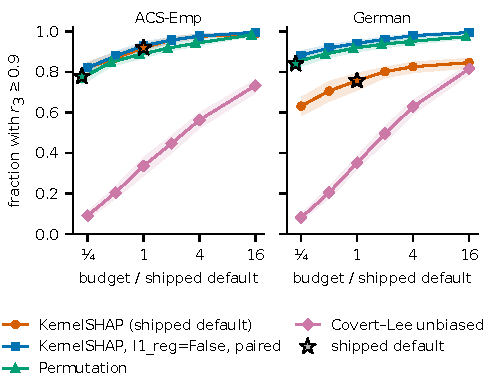
\includegraphics{fig4_budget.pdf}
\caption{\textbf{Reliability against budget: the shipped defaults, and the unbiased estimator that needs far more.}
Fraction of instances with $r_3\ge 0.9$ against the budget in coalitions relative to the shipped KernelSHAP default ($2d+2048$) of the same cell, one panel per dataset (three models, three seeds pooled; 95\% cluster-bootstrap bands).
Markers: shipped defaults (KernelSHAP at $\times1$; Permutation at its own 500 evaluations). Colour = explainer, fixed across figures.}
\label{fig:budget}
\end{figure}

\subsection{Certificates: calibrated, conservative and dear}
\label{sec:exp-cert}

We ask whether a certificate computed from the run itself gives a reliability guarantee at a lower cost than a fixed budget. We test it on the six main cells at $k=3$ and $\delta=0.1$, on fresh reruns, with the run stopped at the first certifying stage (Figure~\ref{fig:cert}, Table~\ref{tab:cert}).

\textbf{Calibration.}
All five rules are calibrated at $\delta=0.1$: among certified runs the exact set is returned at least 0.919 of the time, with every lower confidence limit at or above 0.900. Bonferroni, max-$t$, split-half and SHAP@k-style stopping are conservative: 0.998--1.000 of the certified runs are exact. The plug-in rule that tests only the weakest chosen attribute against the strongest excluded one is close to its limit (0.919--0.942) and breaks at $\delta=0.2$ for $k=5$, where P(exact $\mid$ certified) is 0.764--0.774 in three of the six cells (ACS with logistic regression, ACS with trees, German with logistic regression); this is the winner's curse the corrected rules were built against. Of the 360 combinations of rule, $\delta$, $k$ and cell, 357 are calibrated.

\textbf{Power.}
The price of that safety is abstention. The four conservative rules certify 40--64\% of runs at $k=3$ (10--36\% at $k=5$) and use $2.0$--$2.8\times10^{4}$ coalitions on average, about ten times the default. Against an oracle that certifies exactly when $r_3(x;B)\ge 1-\delta$ (from 200 reruns of 30 instances per cell, stratified by $r$, so that shares are conditional on the strata), Bonferroni and max-$t$ certify 50--80\% of the instances the oracle would certify at $4\times$ the default, and split-half and SHAP@k-style 24--67\%, while the plug-in rule certifies 26--45\% of instances that the oracle would not.

\textbf{Price.}
The comparison depends on what is held fixed. Against the same estimator, stopping on a certificate costs less than running fixed Covert--Lee stages to the same pooled correct rate (21.6k against 33.3k coalitions on ACS with logistic regression; in two cells no fixed stage up to $16\times$ reaches the rate). Against the best fixed alternative it does not: KernelSHAP with $\ell_1$ selection off and paired sampling at a quarter of the default budget (about 520 coalitions, the floor of our grid) already delivers a pooled exact rate of 0.92--0.97, above that of the certified runs (0.85--0.94), at about one fortieth of the cost, in all 24 combinations of rule and cell. The shipped default reaches the certificates' rate only on ACS. We read this as follows: certificates are valid, they give a statement about the run in hand that a fixed rate does not, but their price is high, and on these near-additive tabular models a corrected estimator at a small budget is the cheaper way to a reliable explanation. The grid floor means the saving may be larger.

\begin{figure*}[t]
\centering
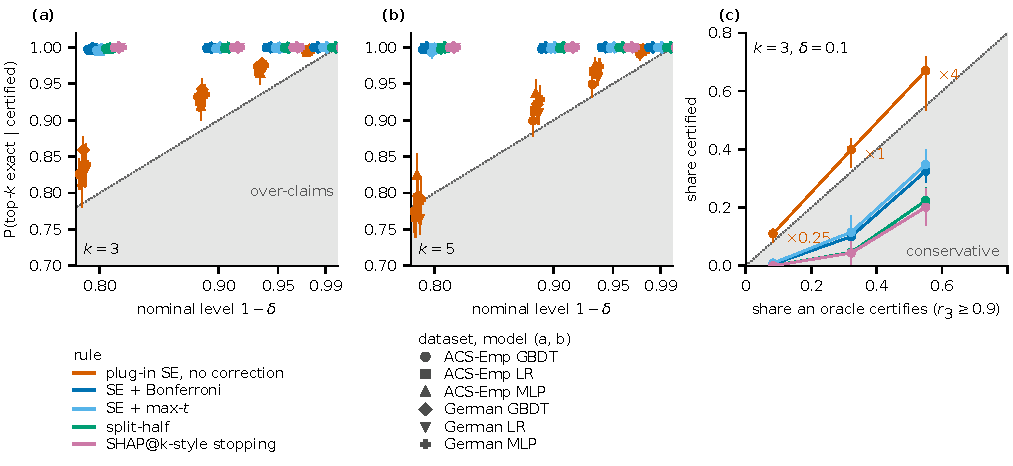
\includegraphics{fig3_certificates.pdf}
\caption{\textbf{In-run certificates are calibrated, and conservative.}
(a, b)~Calibration of the five certificates on fresh reruns, for the top-3 (a) and top-5 (b): $P(\text{top-}k\text{ of the delivered run is exact}\mid\text{certified})$
against the nominal level $1-\delta$, pooled over instances and seeds with 95\% cluster-bootstrap intervals; colour = rule, marker = dataset and model.
On the diagonal = calibrated; above = conservative; below = over-claims.
(c)~Power: share of runs certified by a coalition stage ($\times\tfrac14,\times1,\times4$ of the Covert--Lee schedule) against the share of instances an oracle that knows $r_3(x;B)$ would certify at that stage
($r_3\ge 0.9$, $R\approx 200$ reruns on 30 stratified instances per seed-0 cell; mean over the six cells, bars = range).
Below the diagonal = the certificate gives up power relative to the oracle.}
\label{fig:cert}
\end{figure*}

\begin{table*}[t]
\caption{\textbf{What certification costs and what it gives up} ($k{=}3$, $\delta{=}0.1$). Each cell is the range over the six dataset--model groups (per-group values in Table~\ref{tab:cert-cells}).
\emph{Certificate}: share of fresh runs certified at some stage of the seven-stage schedule; $P(\text{exact}\mid\text{certified})$; correct rate of the delivered run.
\emph{Against the oracle} (stage $\times4$; 30 stratified instances per seed-0 cell, $R\approx 200$; shares are conditional on the strata, not population rates):
share of oracle-certifiable instances the rule certifies, and share of the others it certifies.
\emph{Coalitions to reach the delivered rate}: this certificate, against the cheapest fixed budget on the grid whose pooled $P(\text{top-3 exact})$ reaches that rate,
for the same estimator, for KernelSHAP with \texttt{l1\_reg=False}, and for the shipped KernelSHAP default
($\le$ marks the grid floor; n/a: no fixed budget up to $\times16$ reaches the rate; counts of cells in parentheses).}
\label{tab:cert}
\centering\small
\begin{tabular}{@{}lccccc@{}}
\toprule
 & plug-in SE & Bonferroni & max-$t$ & split-half & SHAP@k \\
\midrule
\multicolumn{6}{@{}l}{\emph{certificate, fresh reruns}} \\
\hspace{0.8em}share of runs certified & 0.78--0.88 & 0.50--0.62 & 0.52--0.64 & 0.44--0.54 & 0.40--0.49 \\
\hspace{0.8em}P(exact $\mid$ certified) & 0.92--0.94 & 1.00 & 1.00 & 1.00 & 1.00 \\
\hspace{0.8em}delivered run correct & 0.87--0.91 & 0.89--0.94 & 0.89--0.94 & 0.85--0.91 & 0.89--0.94 \\
\multicolumn{6}{@{}l}{\emph{share of instances certified at $\times4$ (stratified subset)}} \\
\hspace{0.8em}where the oracle certifies ($r_3\geq 0.9$) & 0.88--0.94 & 0.50--0.78 & 0.55--0.80 & 0.29--0.67 & 0.24--0.66 \\
\hspace{0.8em}where it does not & 0.26--0.45 & 0.00--0.01 & 0.01--0.03 & 0.00--0.02 & 0.00 \\
\multicolumn{6}{@{}l}{\emph{coalitions to reach the delivered rate ($\times10^3$)}} \\
\hspace{0.8em}this certificate & 10--14 & 20--24 & 20--23 & 23--27 & 24--28 \\
\hspace{0.8em}fixed budget, same estimator & 33 & 33 (2 n/a) & 33 (2 n/a) & 33 & 33 (2 n/a) \\
\hspace{0.8em}fixed, KernelSHAP \texttt{l1\_reg=False} & $\leq$0.52 & $\leq$0.52 & $\leq$0.52 & $\leq$0.52 & $\leq$0.52 \\
\hspace{0.8em}fixed, KernelSHAP shipped default & $\leq$0.52 (3 n/a) & $\leq$0.52 (3 n/a) & $\leq$0.52 (3 n/a) & $\leq$0.52 (3 n/a) & $\leq$0.52 (3 n/a) \\
\bottomrule
\end{tabular}

\end{table*}

\subsection{How much budget, and for which instances}
\label{sec:exp-budget}

The shipped estimators leave little room for a per-instance budget: at the default the budget at which an instance first reaches $r_3\ge0.9$ has an interquartile range of at most one octave over instances for KernelSHAP and Permutation, because most instances are satisfied already at the smallest budget we tried (82\% on ACS and 63\% on German Credit for the shipped default) or never reach the target (11--18\% of German instances are still unreliable at $16\times$). The spread is wide for the unbiased estimator, with an interquartile range of two to three octaves at $\delta=0.1$ (16--29\% of instances do not reach the target by $16\times$), and the budget predicted from $c\,\sigma^2/\mathrm{gap}^2$ with one fitted constant per cell ranks instances like the observed one (Spearman 0.91 on each task, over the instances that reach the target). So the dependence of the required budget on the margin is real where the sampling error is the dominant error, which is the estimator whose certificate is audited above, and it is absent where a bias floor sets the error, as in the German default.

\subsection{Rerun noise next to accepted variation}
\label{sec:exp-yardstick}

Whether rerun noise matters is also a question of scale: practitioners already live with changes of the explanation when the background sample is redrawn or the model is retrained. For 30 instances of the first model seed of each cell we compare the disagreement between 20 reruns of the shipped default (mean pairwise one minus top-3 Jaccard) with the disagreement of the \emph{exact} Shapley values across background resamples and across retrains within $0.01$ AUC of the audited model, by seed alone and by bootstrap of the training set (Figure~\ref{fig:yardstick}). A retrain changes the model, so this scale only says whether estimator noise is smaller than variation already accepted. Four of the six cells have been completed (ACS Employment with all three models, German Credit with logistic regression); the German MLP and tree runs are not part of this section.

In none of the four cells is the mean rerun disagreement of the shipped default (0.005--0.052) larger than that of a non-vacuous reference (0.049--0.59). Per instance the answer depends on the reference. Against background resampling the rerun disagreement is strictly smaller for 73--93\% of instances, equal for 7--23\% and larger for at most 7\%, which meets our pre-registered criterion (a strict share of at least 0.75 with a lower confidence limit of at least 0.6) in the three ACS cells and not for German logistic regression (0.73). Against retraining it is strictly smaller for 23--100\% of instances, and the criterion is met only for the ACS MLP (both retrain variants) and for German logistic regression (bootstrap retrain); the remainder are mostly ties in which both disagreements are zero, because for ACS logistic regression and trees the top-3 set of the exact values is itself often unchanged by a retrain. Estimator noise of the shipped default is therefore not a larger source of variation than the changes practitioners accept, but this says little about whether a given run is right. On German Credit the rerun disagreement is small and the run is still wrong (Section~\ref{sec:exp-default}), because the error is shared by all reruns.

\begin{figure}[t]
\centering
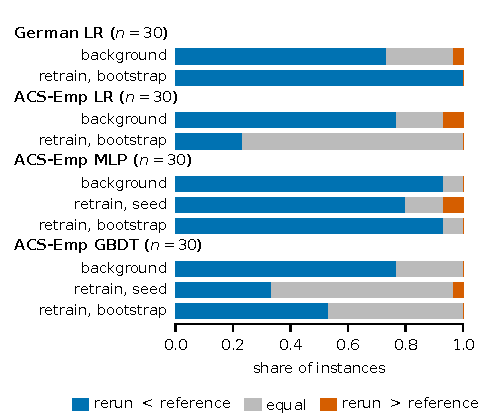
\includegraphics{fig2_yardstick.pdf}
\caption{\textbf{Rerun noise of the shipped KernelSHAP against variation practitioners already accept.}
For each instance, the disagreement between reruns of the explainer (mean pairwise $1-$ top-3 Jaccard over $R{=}20$ runs) is compared with the disagreement of the
\emph{exact} Shapley values across background resamples, across retrains that differ in the seed only, and across bootstrap retrains of the training set
(retrains within $0.01$ AUC of the audited model). Bars: share of instances where the rerun disagreement is smaller than (blue), equal to (grey) or larger than (orange) the reference; ties are mostly $0=0$.
Seed-only retraining of the logistic regression is deterministic, so that bar is absent. 30 instances per cell, model seed 0; four of the six cells.}
\label{fig:yardstick}
\end{figure}

\subsection{Controls}
\label{sec:exp-controls}

A practitioner who summarises \emph{global} importance sees none of this. The global top-3 set by mean $|\phi|$ over the 100 instances, computed from one run per instance, equals the exact global top-3 in every one of the 20 reruns on every cell, while the mean single-instance $r_3$ at the default budget is 0.77--0.98 on the same instances; a global check does not detect instance-level unreliability. A random $k$-set is exact with probability below 0.002 for $k=3$. Per-instance calls from 20 reruns agree with those from 200 reruns in 97\% of the cases on average (minimum 77\%).

\section{Discussion and Limitations}
\label{sec:discussion}

\textbf{Is one run enough?}
Our answer depends on the configuration. A single run of KernelSHAP with $\ell_1$ selection off and paired sampling at a small budget returns the exact top-3 set in at least nine of ten runs for 92--95\% of instances on every cell of both tasks (Table~\ref{tab:reliable}), so for the models we tested one run of a corrected estimator is a reasonable basis for a top-3 explanation. The shipped default is not at $d=20$, and its failure cannot be seen from reruns. On ACS the shipped default is adequate on average, but a few percent of instances remain whose exact set is unstable; they are near ties, so the instability is a statement about the size of the gap and not about the quality of the explanation. A deployer cannot see which instances these are from a shipped run, and a certificate that identifies them is correct when it speaks but silent on many instances that were fine.

\textbf{What this suggests, where measured.}
For $d\ge11$ the library's default selection rule should not be used unexamined: the exact top-3 differs in a way no rerun reveals, and budget does not repair it. A fixed, corrected estimator at a small budget is a better first choice than a certificate for our models; a certificate is warranted when a per-run statement is itself required, for example for documentation, and then a Bonferroni or max-$t$ rule is the best of those we tested.

\textbf{Limitations.}
We study the interventional Shapley value, two tabular tasks with $d\le20$ in the main grid, a logistic regression, a small MLP and gradient-boosted trees, and 100 instances per cell, with the reference computed by enumeration; the results need not carry over to larger $d$ (one supplementary check up to $d=100$ is in Appendix~\ref{app:extra}), to conditional Shapley values or to other model classes and datasets. The budget grid starts at a quarter of the default, so the saving of a small fixed budget over a certificate may be understated. Oracle shares use a subset of 30 instances per cell stratified by $r_3$, and are shares within strata. Certification was audited on exact value tables only. Random forests, the sampling explainer and a background-size sweep were not run.


\section*{AI Disclosure Statement}
This study was carried out by a group of generative-AI (large language model) agents working with tool access and no human in the loop during the work. The agents proposed the research question and design, searched and read the literature, wrote the experiment and analysis code, ran the experiments, produced the figures and tables, interpreted the results and drafted all of the text. No generative-AI system is part of the method under study; the explainers and models evaluated are standard tabular learners and Shapley estimators. All numbers in this paper are produced by the released code, and every reference was checked against bibliographic metadata.


\section*{Impact Statement}
Feature attributions are used to justify decisions about credit, health and similar matters, often from a single run of a randomised estimator. Our results indicate when such a run can and cannot be relied on, and what a deployer can check from the run itself. A possible harm is over-trust in an explanation that has passed one of the checks we examine; we therefore report where those checks fail. The study uses public data only and explains models trained on them; the credit and census data concern people, and we use them as released.


\bibliography{refs}
\bibliographystyle{icml2027}

\appendix
\onecolumn
\section{Validity of the re-implemented estimators}
\label{app:e0}

All arms are run on a table of exact coalition values so that $10^5$ reruns remain affordable, which requires re-implementing the estimators. Before any result was produced we compared the re-implemented KernelSHAP at its shipped default with the library's own explainer on four settings: German Credit with an MLP ($d=20$), ACS Employment with an MLP and with gradient-boosted trees ($d=16$), and German Credit with logistic regression restricted to $d=10$, where the library enumerates all coalitions. Six instances were rerun 100 times per setting. In the three sampled settings the top-1 hit rates are identical, the top-3 and top-5 hit rates differ by at most 0.13 (binomial standard error of a difference at most 0.07), the per-attribute mean differs by at most 3.1 standard errors, and the ratio of rerun standard deviations lies between 0.96 and 1.04. In the enumerated setting both return the exact value to numerical precision. We read this as agreement of the two implementations in distribution, with the remaining per-attribute mean differences, up to 3.1 standard errors over many attributes, not separately explained.


\section{Additional results}
\label{app:extra}

\paragraph{Beyond $d=20$.}
A supplementary check on one further dataset (Arrhythmia, gradient-boosted trees on the margin scale, one seed, 20 instances) uses the interventional TreeSHAP value as the exact reference, so that $d$ is not limited by enumeration. At $d=40$ (a subset of the attributes) and $d=100$, the shipped KernelSHAP default returns the exact top-3 in a mean of $0.55$ and $0.49$ of the reruns at the shipped budget, and between $0.33$ and $0.58$ at every budget from a quarter to $16\times$ the shipped one. Paired \texttt{l1\_reg=False} reaches $0.98$--$1.00$ at the shipped budget and above, and Permutation with 500 evaluations $0.94$ and $0.96$. The $\ell_1$ truncation is therefore not specific to German Credit and does not vanish above $d=20$; with one model, one seed and 20 instances this checks that, and does not estimate how much of it a typical task shows.

\begin{figure}[h]
\centering
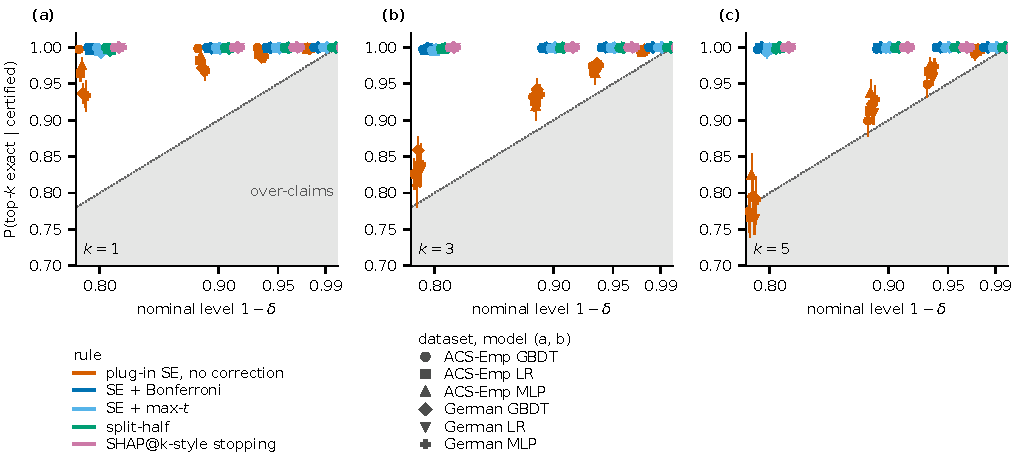
\includegraphics{figA_calibration_k135.pdf}
\caption{Calibration of the certificates for $k=1,3,5$ (as Figure~\ref{fig:cert}a,b).}
\label{fig:cal-k135}
\end{figure}

\begin{figure}[h]
\centering
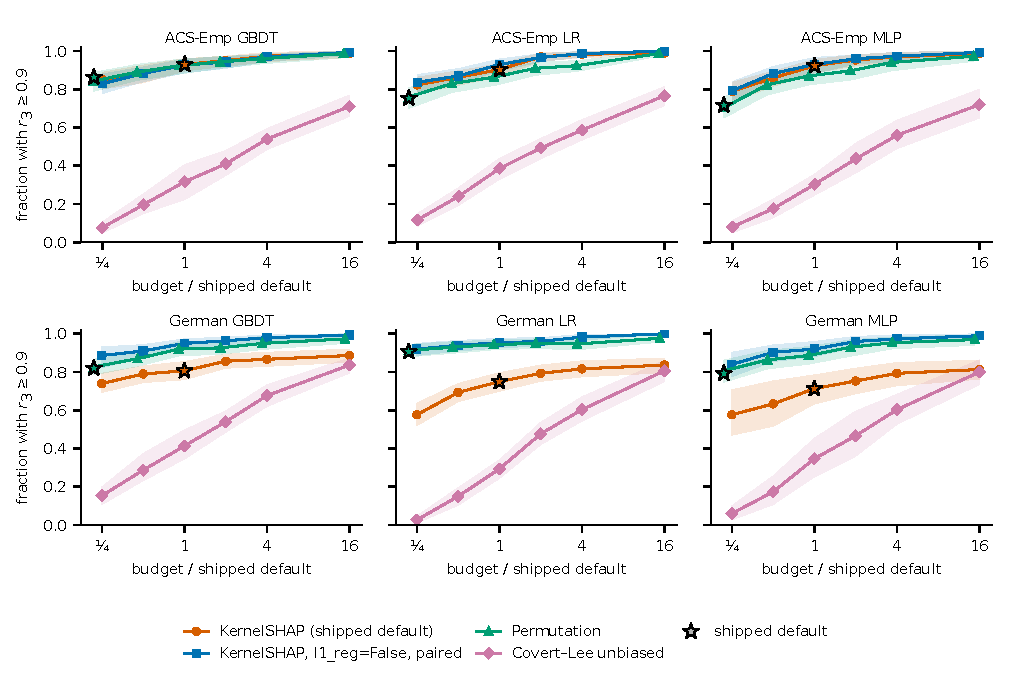
\includegraphics{figA_budget_by_model.pdf}
\caption{As Figure~\ref{fig:budget}, with one panel per dataset and model.}
\label{fig:budget-model}
\end{figure}

\begin{figure}[h]
\centering
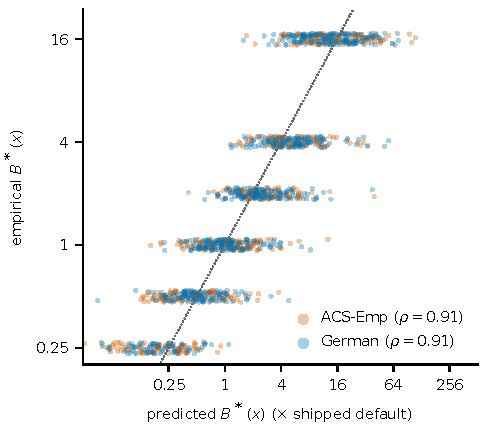
\includegraphics{figA_bstar.pdf}
\caption{Required budget $B^*(x)$ per instance: predicted from $c\sigma^2/\mathrm{gap}^2$ ($c$ fitted per cell) against the smallest grid budget at which $r_3\ge0.9$ (Covert--Lee, $k=3$, $\delta=0.1$). Instances not reliable by $16\times$ are censored there and drawn hollow. Spearman rank correlation over uncensored points in the legend.}
\label{fig:bstar}
\end{figure}

\begin{figure}[h]
\centering
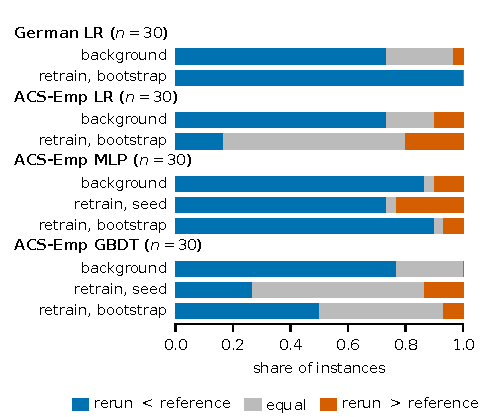
\includegraphics{fig2_yardstick_perm.pdf}
\caption{As Figure~\ref{fig:yardstick}, for the Permutation explainer.}
\label{fig:yardstick-perm}
\end{figure}

\begin{figure}[h]
\centering
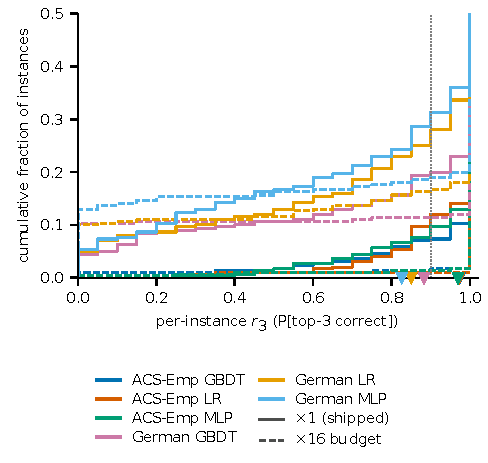
\includegraphics{figA_ecdf_x16.pdf}
\caption{Exact $r_3$ at the shipped budget (solid) and at $16\times$ that budget (dashed), as Figure~\ref{fig:tail}a.}
\label{fig:ecdf16}
\end{figure}

\begin{figure}[h]
\centering
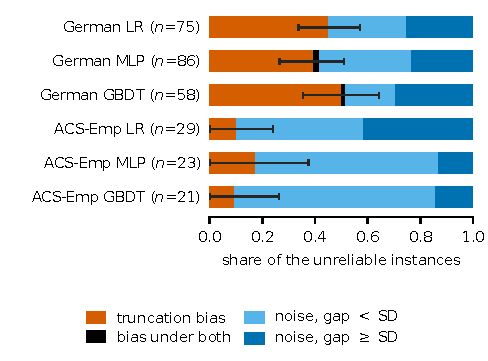
\includegraphics{figA_c5_split.pdf}
\caption{What the unreliable instances of the shipped KernelSHAP default are made of. Per cell group (three seeds pooled), the instances with $r_3<0.9$ at the shipped budget ($n$ in the labels) split by the \emph{mean} attribution of the default's reruns: wrong top-3 under the default but right under paired \texttt{l1\_reg=False} (truncation bias; 95\% cluster-bootstrap interval); wrong under both; right but the runs scatter (noise), split by the gap between the $3$rd and $4$th attribution against the rerun SD of that difference ($z_{\rm true}$ below / at or above 1; a descriptive threshold). Interval widths reflect small $n$ on ACS.}
\label{fig:c5}
\end{figure}

\begin{table}[h]
\caption{Per-cell values behind Table~\ref{tab:cert}.}
\label{tab:cert-cells}
\centering\scriptsize
\begin{tabular}{@{}llccccrr@{}}
\toprule
Dataset, model & Rule & certified & P(exact $\mid$ certified) & delivered correct & coalitions & fixed Covert--Lee & fixed \texttt{l1\_reg=False} \\
\midrule
ACS-Emp GBDT & plug-in SE & 0.78 & 0.932 [0.920, 0.944] & 0.87 & 14148 & 33280 & $\leq$520 \\
 & Bonferroni & 0.50 & 0.999 [0.998, 1.000] & 0.89 & 22955 & n/a & $\leq$520 \\
 & max-$t$ & 0.52 & 0.998 [0.996, 1.000] & 0.89 & 22366 & n/a & $\leq$520 \\
 & split-half & 0.44 & 0.999 [0.997, 1.000] & 0.85 & 25288 & 33280 & $\leq$520 \\
 & SHAP@k & 0.41 & 1.000 [1.000, 1.000] & 0.89 & 25828 & n/a & $\leq$520 \\
\addlinespace[2pt]
ACS-Emp LR & plug-in SE & 0.84 & 0.926 [0.912, 0.937] & 0.89 & 11019 & 33280 & $\leq$520 \\
 & Bonferroni & 0.57 & 0.999 [0.998, 1.000] & 0.92 & 21551 & 33280 & $\leq$520 \\
 & max-$t$ & 0.58 & 0.998 [0.996, 1.000] & 0.92 & 20928 & 33280 & $\leq$520 \\
 & split-half & 0.50 & 0.999 [0.997, 1.000] & 0.88 & 24141 & 33280 & $\leq$520 \\
 & SHAP@k & 0.46 & 1.000 [1.000, 1.000] & 0.92 & 25241 & 33280 & $\leq$520 \\
\addlinespace[2pt]
ACS-Emp MLP & plug-in SE & 0.82 & 0.919 [0.900, 0.937] & 0.87 & 12436 & 33280 & $\leq$520 \\
 & Bonferroni & 0.52 & 0.999 [0.997, 1.000] & 0.90 & 23182 & n/a & $\leq$520 \\
 & max-$t$ & 0.54 & 0.998 [0.996, 1.000] & 0.90 & 22508 & n/a & $\leq$520 \\
 & split-half & 0.44 & 1.000 [1.000, 1.000] & 0.87 & 25703 & 33280 & $\leq$520 \\
 & SHAP@k & 0.40 & 1.000 [1.000, 1.000] & 0.90 & 26685 & n/a & $\leq$520 \\
\addlinespace[2pt]
German GBDT & plug-in SE & 0.88 & 0.942 [0.927, 0.957] & 0.91 & 9647 & 33408 & $\leq$522 \\
 & Bonferroni & 0.62 & 0.999 [0.998, 1.000] & 0.94 & 20218 & 33408 & $\leq$522 \\
 & max-$t$ & 0.64 & 0.999 [0.998, 1.000] & 0.94 & 19561 & 33408 & $\leq$522 \\
 & split-half & 0.54 & 0.999 [0.997, 1.000] & 0.91 & 22919 & 33408 & $\leq$522 \\
 & SHAP@k & 0.49 & 1.000 [1.000, 1.000] & 0.94 & 24092 & 33408 & $\leq$522 \\
\addlinespace[2pt]
German LR & plug-in SE & 0.85 & 0.933 [0.918, 0.945] & 0.90 & 12136 & 33408 & $\leq$522 \\
 & Bonferroni & 0.55 & 0.999 [0.998, 1.000] & 0.92 & 23782 & 33408 & $\leq$522 \\
 & max-$t$ & 0.57 & 0.999 [0.998, 1.000] & 0.92 & 23097 & 33408 & $\leq$522 \\
 & split-half & 0.45 & 1.000 [1.000, 1.000] & 0.90 & 26943 & 33408 & $\leq$522 \\
 & SHAP@k & 0.40 & 1.000 [1.000, 1.000] & 0.92 & 28187 & 33408 & $\leq$522 \\
\addlinespace[2pt]
German MLP & plug-in SE & 0.83 & 0.935 [0.918, 0.949] & 0.89 & 12118 & 33408 & $\leq$522 \\
 & Bonferroni & 0.56 & 0.999 [0.998, 1.000] & 0.92 & 22969 & 33408 & $\leq$522 \\
 & max-$t$ & 0.58 & 0.999 [0.998, 1.000] & 0.92 & 22348 & 33408 & $\leq$522 \\
 & split-half & 0.47 & 1.000 [1.000, 1.000] & 0.89 & 26039 & 33408 & $\leq$522 \\
 & SHAP@k & 0.42 & 1.000 [1.000, 1.000] & 0.92 & 27280 & 33408 & $\leq$522 \\
\bottomrule
\end{tabular}

\end{table}


\end{document}
